\documentclass[UTF8]{ctexbeamer}

\usepackage{zhlipsum}

\usepackage{graphicx}
% 图片位置
\usepackage{float}
% 并排
\usepackage{subfigure}
\usepackage{parskip}

\usetheme{AnnArbor}
\usecolortheme{spruce}

\setbeamerfont{headline}{family=\kaishu}
\setbeamerfont{footline}{family=\kaishu}
\setbeamerfont{frametitle}{family=\kaishu}

% 设置封面校名标题
% 设置背景
\titlegraphic{
\includegraphics[height=1.5cm]{img/hzau-logo.eps}}
\setbeamertemplate{background}{
\includegraphics[width=12.8cm]{img/background.jpg}}

\setbeamerfont{title}{size=\large}
\setbeamerfont{subtitle}{size=\small}
\setbeamerfont{author}{size=\small}
\setbeamerfont{date}{size=\small}
\setbeamerfont{institute}{size=\small}

\definecolor{darkGreen}{RGB}{0, 81, 40}
\definecolor{myGreen}{RGB}{153, 193, 173}
\definecolor{lightGreen}{RGB}{216, 232, 224}

\setbeamercolor*{palette primary}{bg=lightGreen}
\setbeamercolor*{palette secondary}{bg=myGreen, fg = white}
\setbeamercolor*{palette tertiary}{bg=darkGreen, fg = white}

\setbeamercolor*{titlelike}{fg=darkGreen}
\setbeamercolor*{title}{bg=darkGreen, fg = white}
\setbeamercolor*{item}{fg=darkGreen}
\setbeamercolor*{caption name}{fg=darkGreen}
\usefonttheme{professionalfonts}

\usepackage{natbib}

\usepackage{hyperref}
\hypersetup{
	colorlinks=true,
	linkcolor=black,
	citecolor=black
}

\author[张子栋~张敦彪~颜旭~姚代洪]{水哥微生物小队\\张子栋~张敦彪~颜旭~姚代洪}

\title[大豆根系微生物的基因鉴定与基因功能预测]{大豆根系微生物的基因鉴定与基因功能预测}
\subtitle{第九届生物信息设计与技能竞赛}
\institute[HZAU CoI]{华中农业大学
	
	信息学院}
\date{2023年9月27日}

\AtBeginSection[]
{
	\begin{frame}{}
		\transfade
		\tableofcontents[sectionstyle=show/shaded,subsectionstyle=show/shaded/hide]
		\addtocounter{framenumber}{0}
	\end{frame}
}

% \listfiles
\begin{document}

	\kaishu

% ----------------- Frame -----------------

	\begin{frame}
		\titlepage
		
	\end{frame}

% ----------------- Frame -----------------


	\begin{frame}
		\frametitle{目录}
		\tableofcontents
	\end{frame}

% ----------------- Frame -----------------

	\section{背景}
	\begin{frame}{背景}
		\begin{itemize}
			\item 根系微生物\\ \qquad 根系微生物可以对植物生长和健康产生积极影响。研究根系微生物对于促进植物生长健康、提高作物产量质量、维护土壤生态系统健康以及发掘新的生物资源具有重要意义。
			\item 高通量培养\\ \qquad 一种用于微生物培养和筛选的技术,通过该技术可以大大提高微生物的培养效率和筛选速率。
			\item 16S rRNA 物种鉴定与功能预测 \\ \qquad 16S rRNA 序列由高度保守的不可变区和相对可变的可变区组成,可以将研究序列与 16S rRNA 数据库中的序列进行比对,确定研究序列与已知物种或菌株的相似性,并进行进一步的鉴定。
		\end{itemize}
	
	\end{frame}

% ----------------- Frame -----------------

	\section{湿实验过程}
	\begin{frame}{湿实验过程}
		\vspace{0.5cm}
		\begin{columns}
			\column{0.6\textwidth}
			\begin{enumerate}
				\item 培养基制作
				\item 获取大豆根系菌群
				\item 分液与流式细胞分选
				\item PCR 扩增与电泳鉴定
				\item 产物回收与浓度测定
			\end{enumerate}

			\column{0.4\textwidth}
		
		\end{columns}

		\begin{figure}
			\centering
			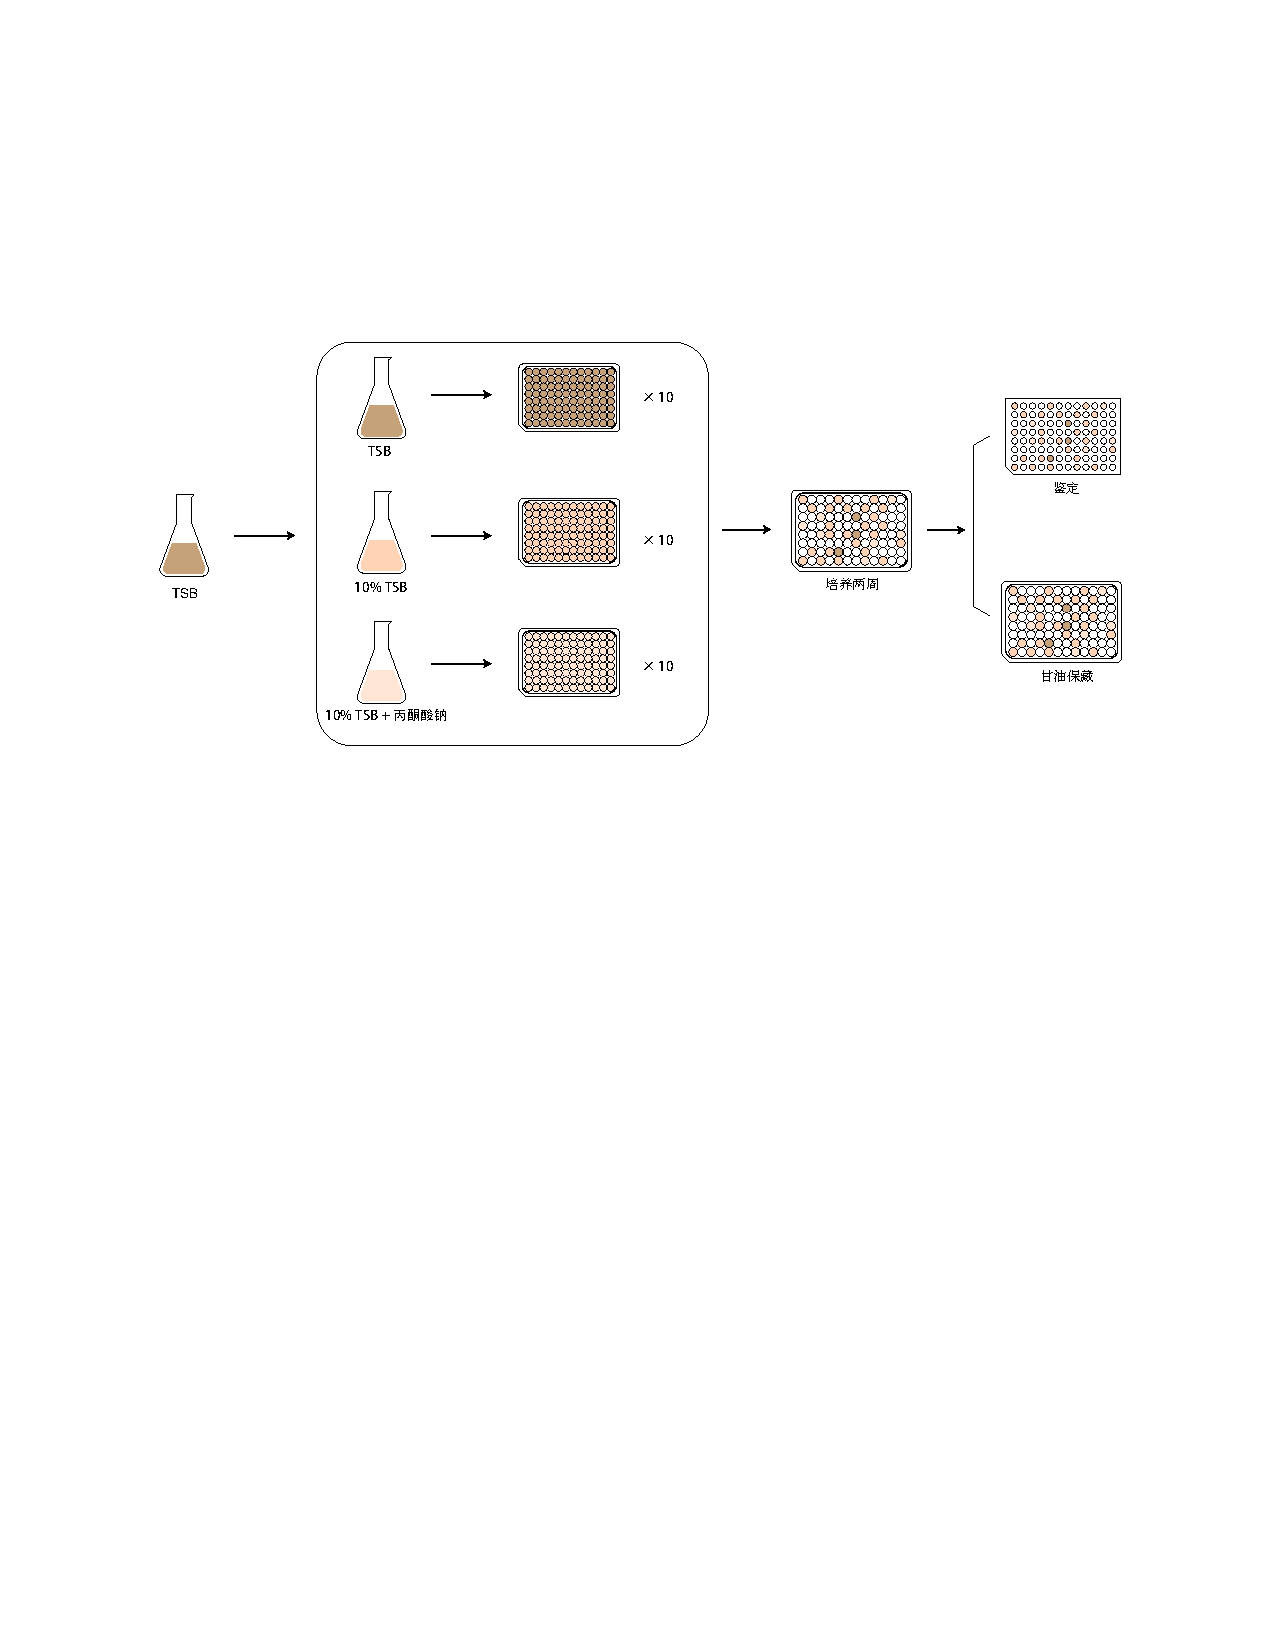
\includegraphics[width=0.8\textwidth]{img/CulturePipeline.pdf}
			\caption{高通量培养}
		\end{figure}
	\end{frame}

% ----------------- Frame -----------------

	\section{数据分析}

	\subsection{数据预处理}
	\begin{frame}{数据分析}{数据预处理}
		\qquad 通过合并双端序列、拆分标签序列和引物序列获得扩增子序列进行后续的生信分析。

		\begin{figure}
			\centering
			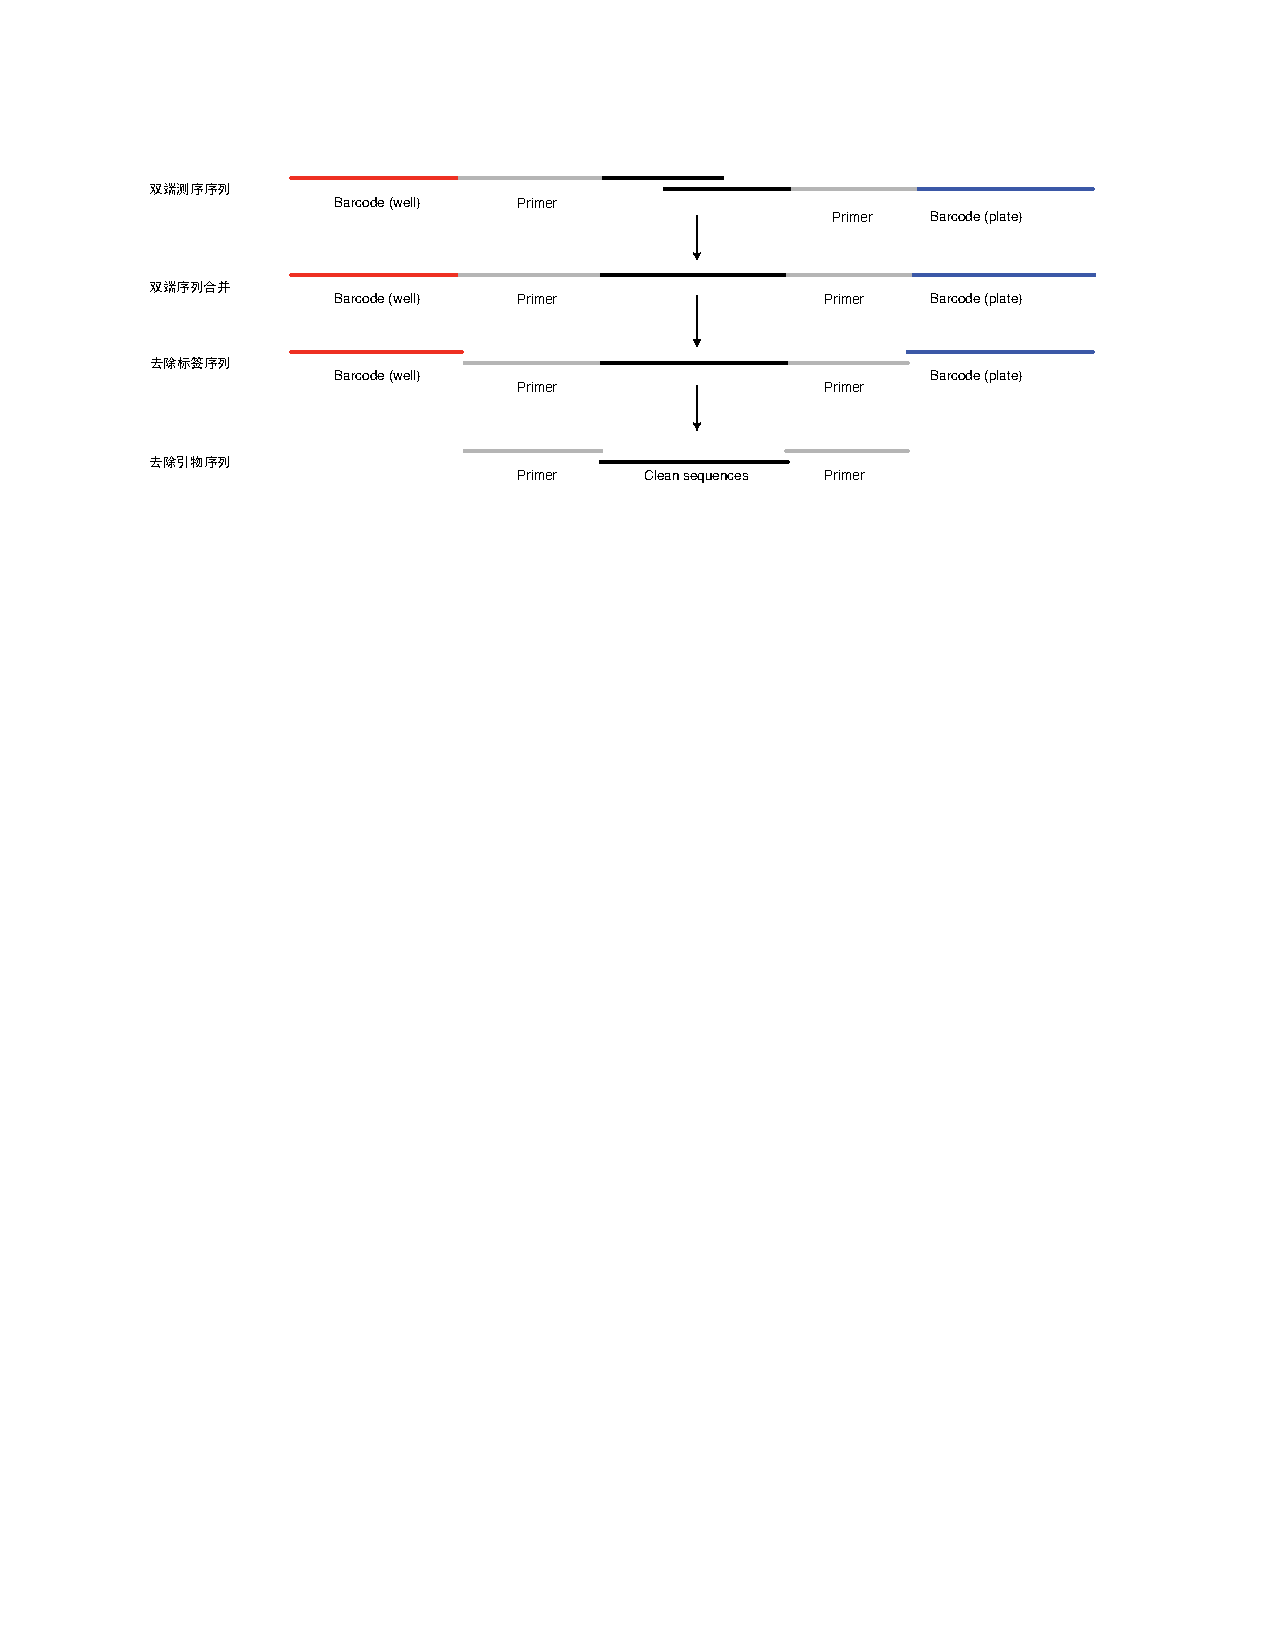
\includegraphics[width=0.98\textwidth]{img/数据预处理.pdf}
			\caption{数据预处理流程}
		\end{figure}
	\end{frame}

% ----------------- Frame -----------------

	\subsection{物种鉴定}
	\begin{frame}{物种鉴定}{流程}

		\begin{enumerate}
			\item 去除重复序列,获得序列丰度
			\item 降噪(UNOISE 算法)鉴定 ASV,从头($de~novo$)去除嵌合体
			\item 构建 ASV 表并基于 RDP 数据库进行物种注释
		\end{enumerate}

		\begin{figure}
			\centering
			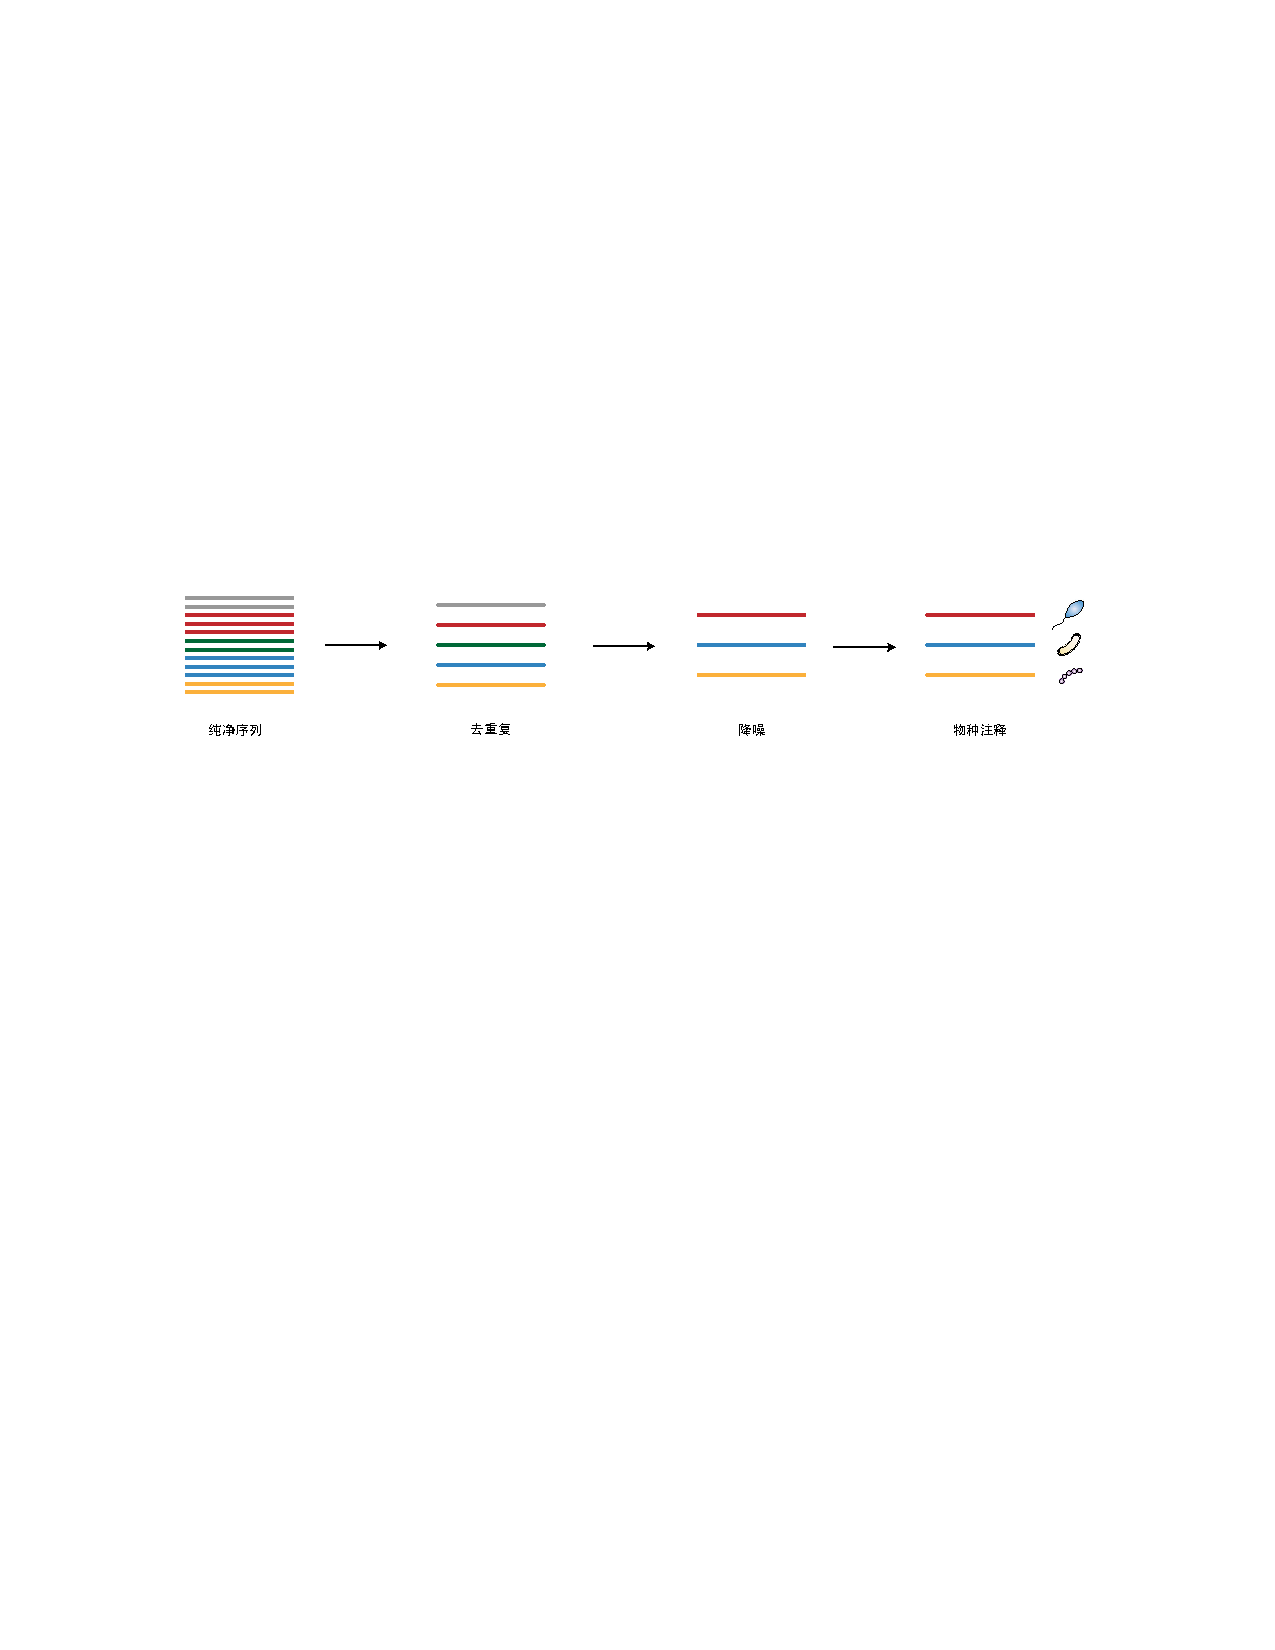
\includegraphics[width=\textwidth]{img/分析流程.pdf}
		\end{figure}
		

	\end{frame}

	% 首先对获取去掉标签和引物后的纯净序列去除重复 获得序列丰度
	% 然后降噪 简化研究对象 获得准确结果
	% 最后进行物种注释 鉴定是哪一种细菌
% ----------------- Frame -----------------

	\begin{frame}{物种鉴定}{挑选代表性序列}
		\begin{columns}
			\column{0.5\textwidth}
			\begin{itemize}
				\item OTU {\tiny (Operational Taxonomic Units)} \\ \qquad OTU 是一种聚类方式,通常在 97\% 的相似水平下聚类生成 OTU,选择每个聚类群中最高丰度序列作为代表性序列。
			\end{itemize}

			\column{0.5\textwidth}
			\begin{itemize}
				\item ASV {\tiny (Amplicon Sequence Variants)} \\ \qquad ASV 则在 100\% 相似水平进行聚类,精度更高,结合降噪算法去除噪声序列所以在增加样本时,结果具有一致性。
			\end{itemize}
		\end{columns}

		\begin{figure}
			\centering
			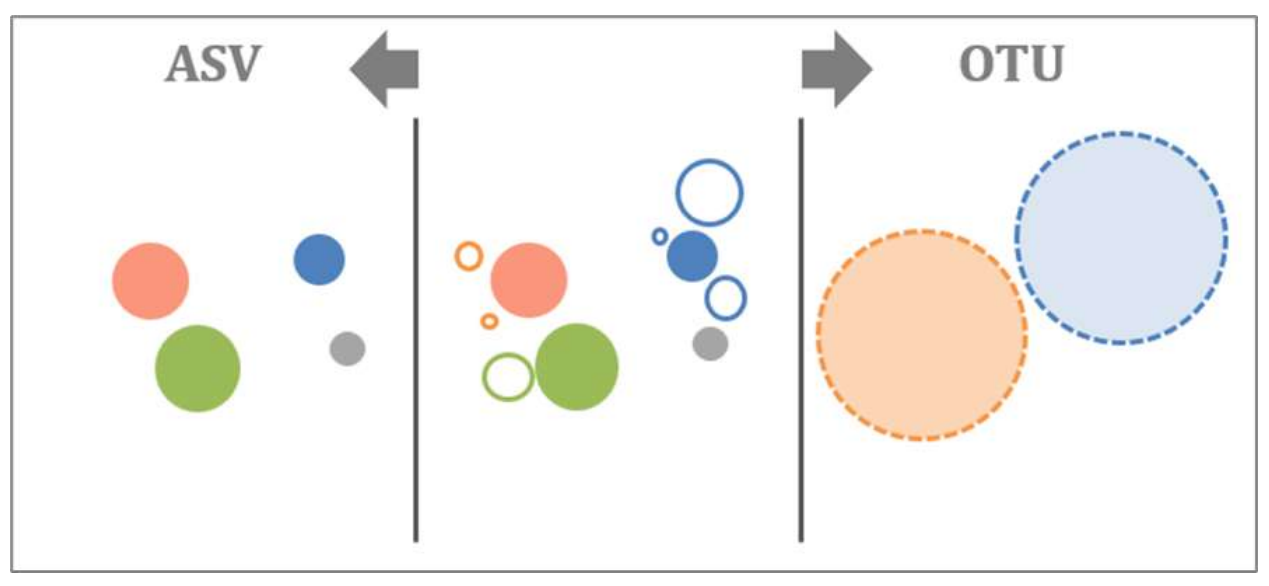
\includegraphics[width=0.7\textwidth]{img/OTUvsASV.png}
		\end{figure}
	\end{frame}

% ----------------- Frame -----------------

	\begin{frame}{物种鉴定}{物种注释}
		\qquad 在挑选代表序列并从头($de~novo$)去除嵌合体后,进行物种注释(基于 RDP 数据库),构建 ASV 表。

		\begin{figure}
			\centering
			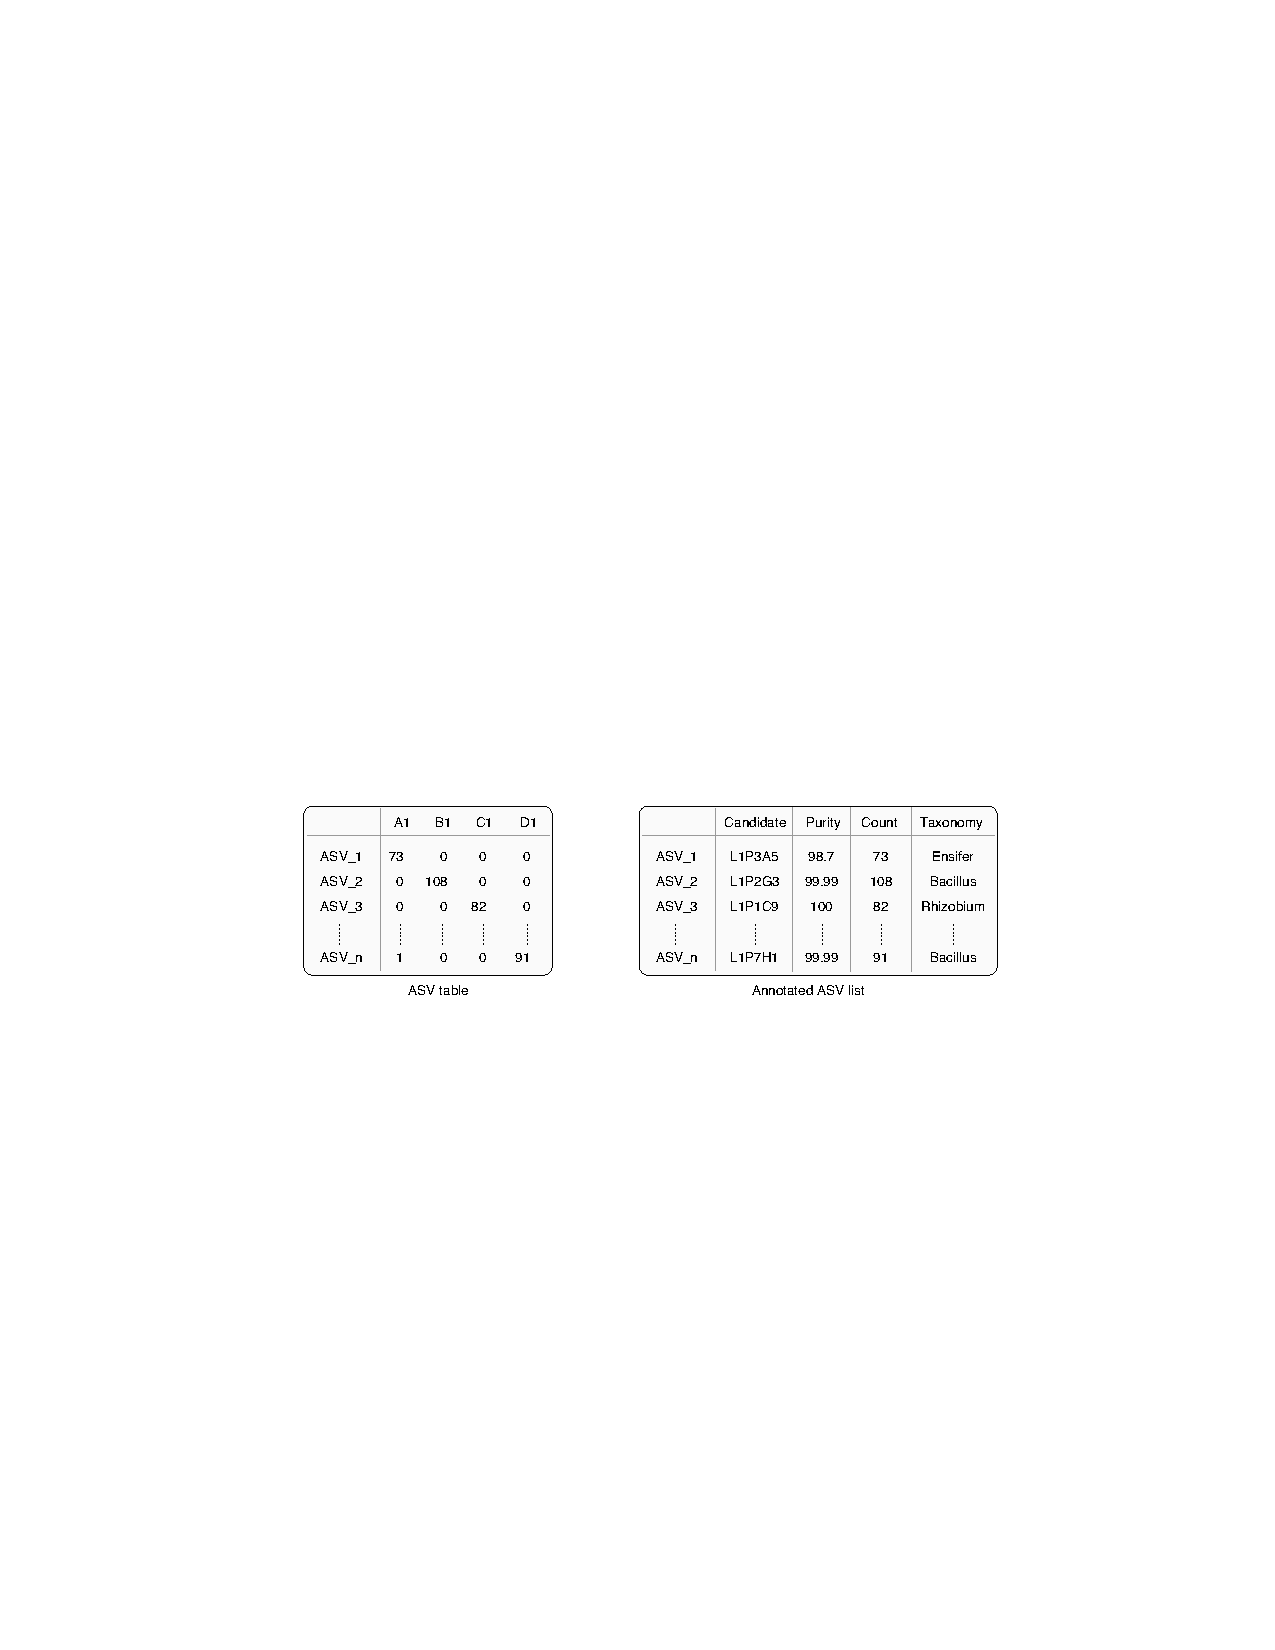
\includegraphics[width=\textwidth]{img/ASVtable.pdf}
		\end{figure}

	\end{frame}

% ----------------- Frame -----------------

	\begin{frame}{物种鉴定}{物种树}
		\qquad 基于 ASV 表绘制物种树。

		\begin{figure}
			\subfigure[根内菌种]{
				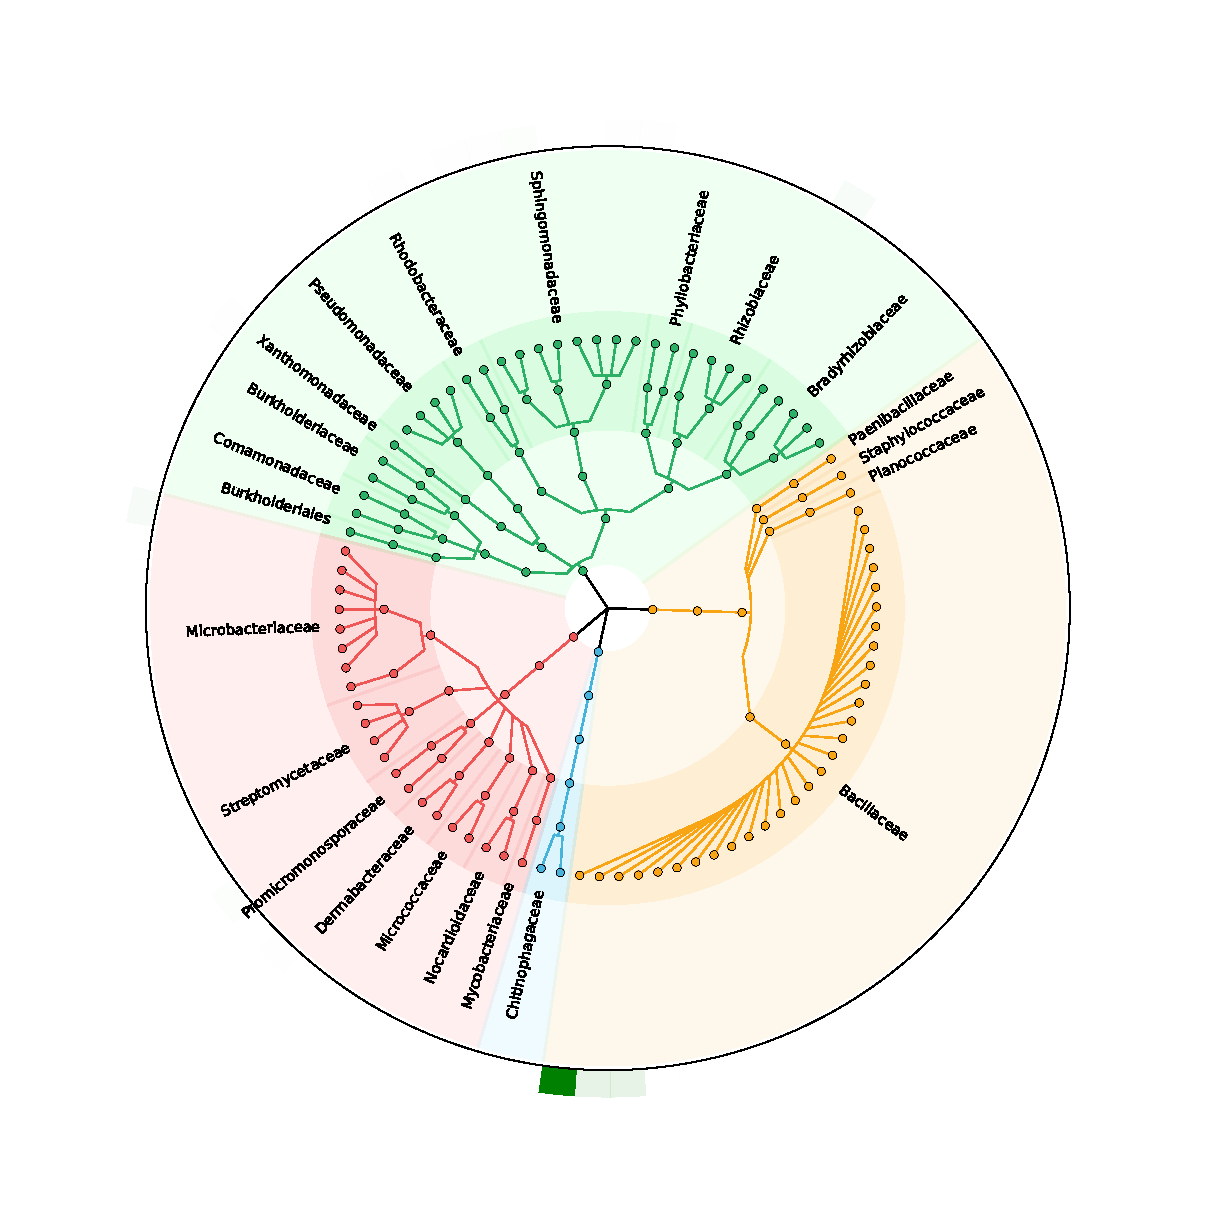
\includegraphics[width=0.45\textwidth]{img/en_graphlan.pdf}
				}
			\subfigure[根际菌种]{
				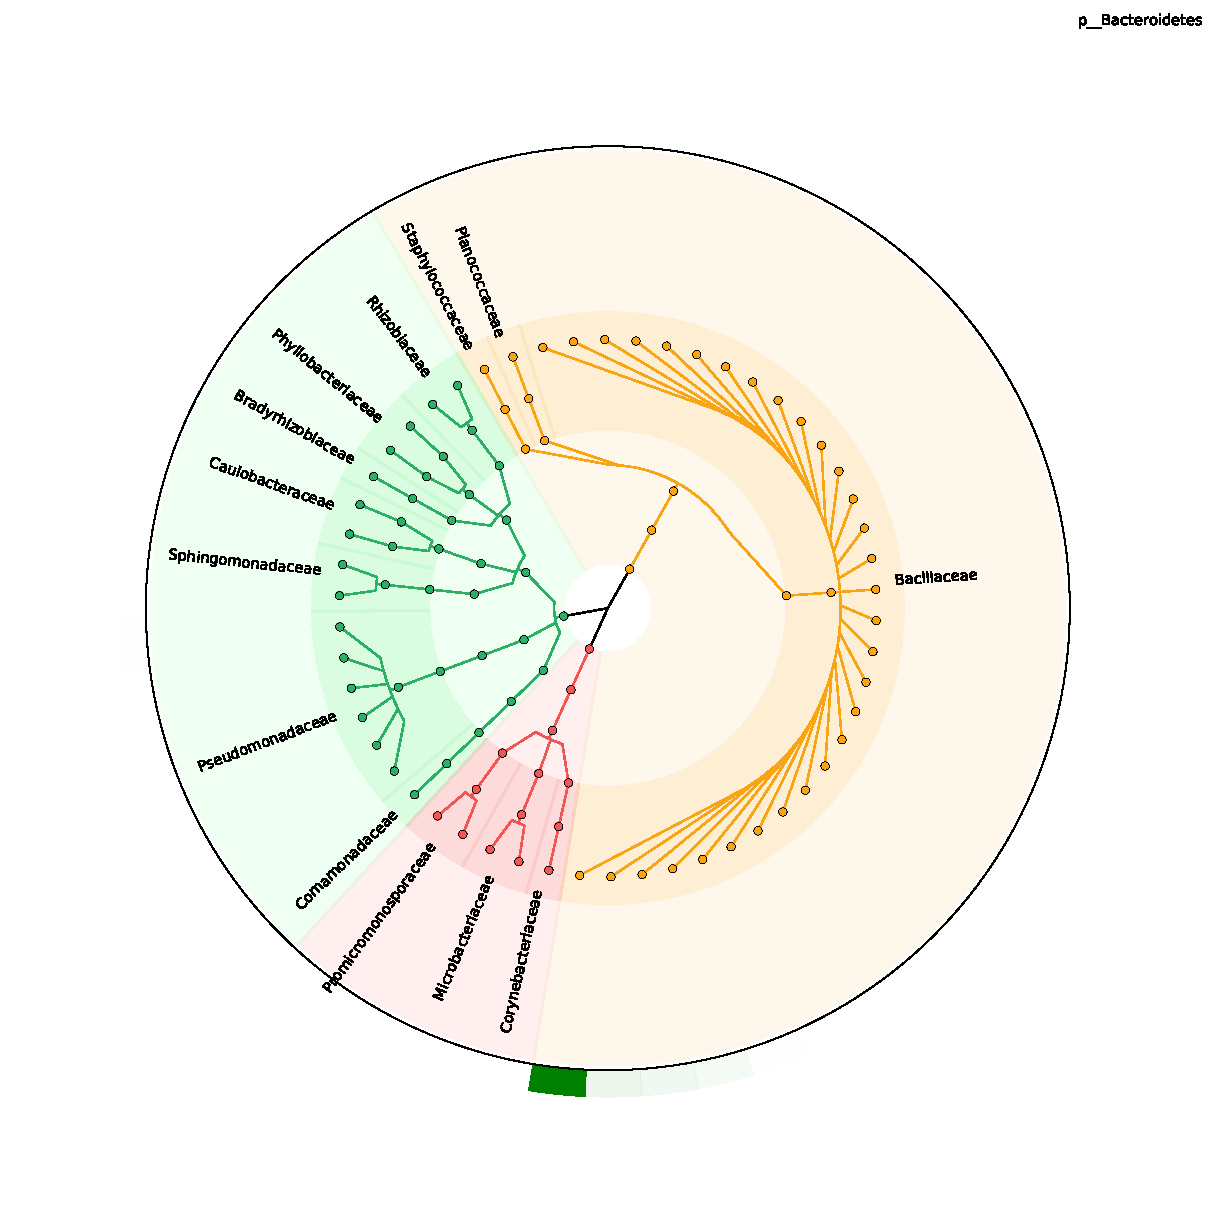
\includegraphics[width=0.45\textwidth]{img/rhi_graphlan.pdf}
				}
		\end{figure}

	\end{frame}


% ----------------- Frame -----------------
	\subsection{功能预测}
	\begin{frame}{功能预测}
		\qquad 使用 PICRUSt2 进行功能预测(ASV 序列、丰度文件作为输入),预测基于多个基因家族数据库(KEGG同源基因、KO直系同源物、EC酶分类编号)。结果使用 R 包 ggpicrust2 进行可视化。
		\begin{figure}
			\centering
			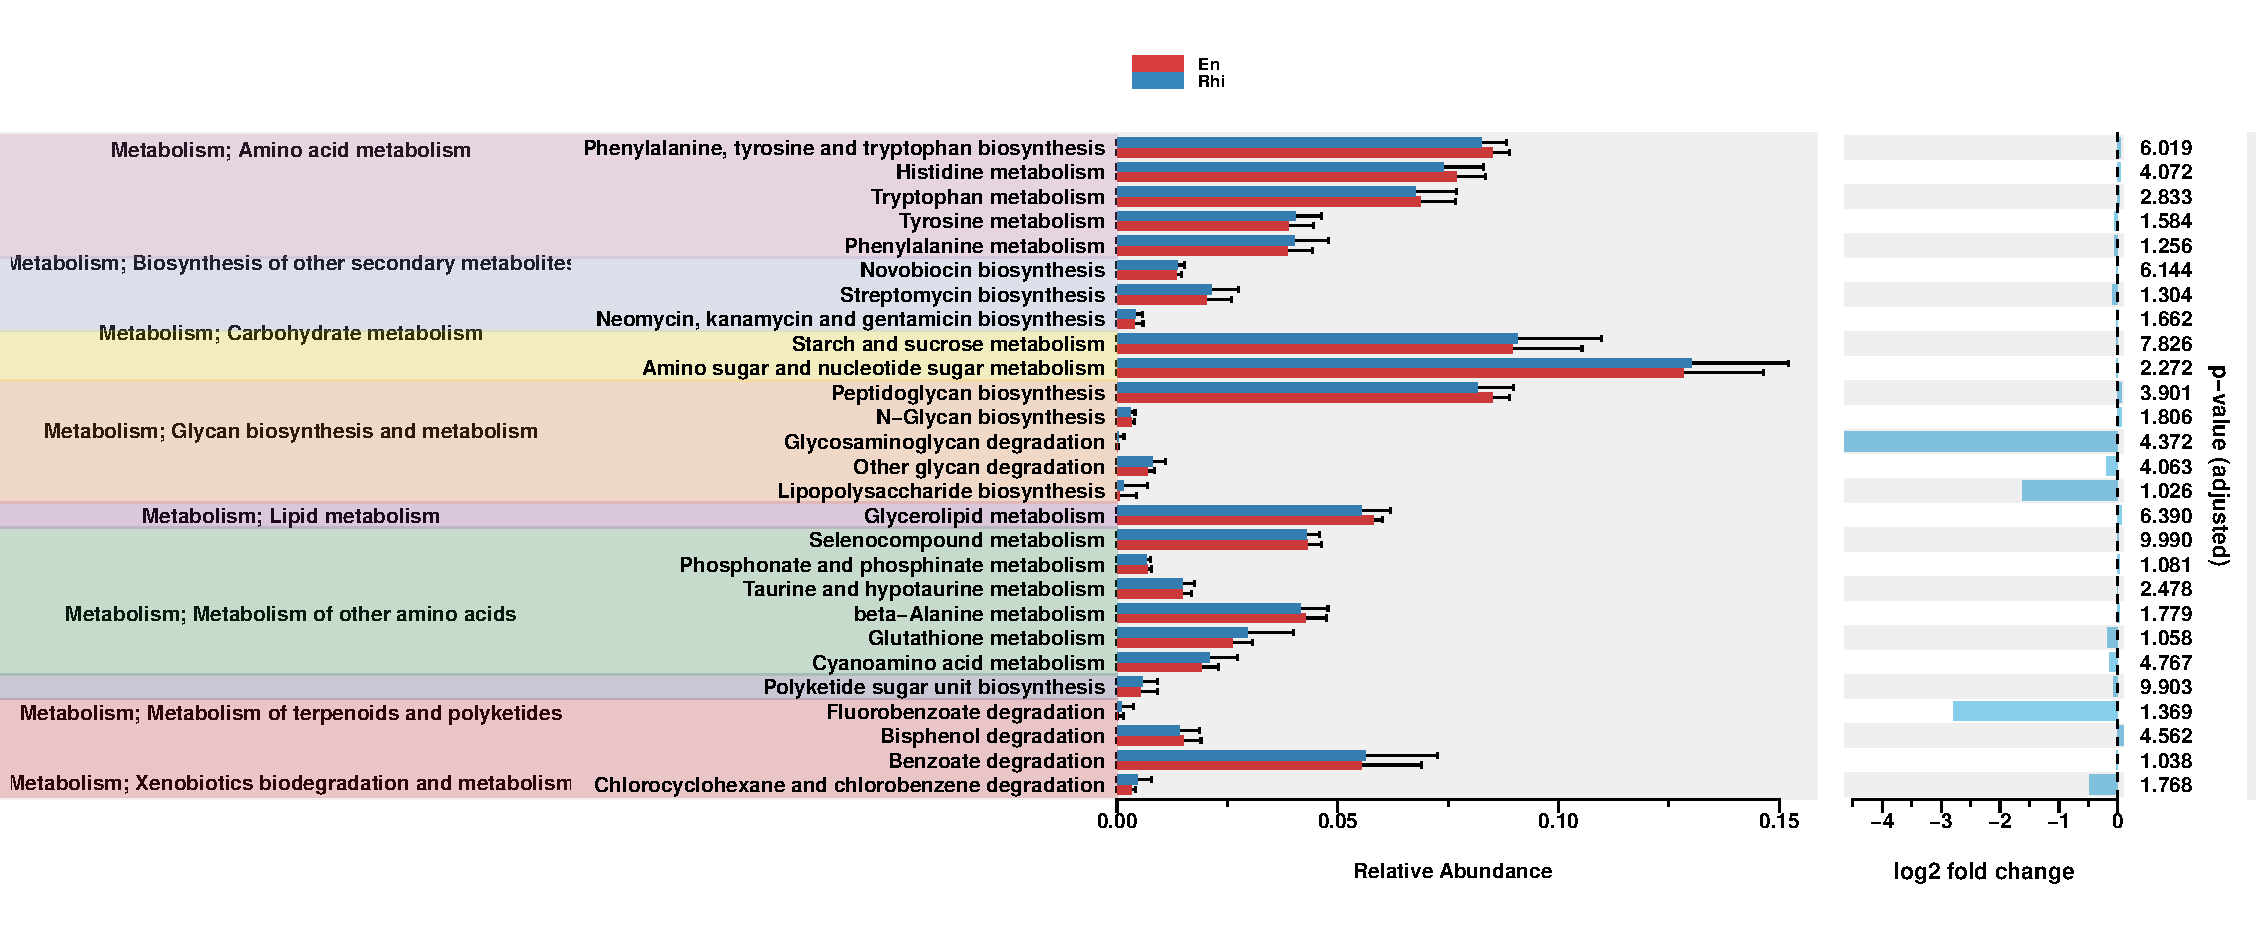
\includegraphics[width=\textwidth]{img/RelativeAbundance60.pdf}
			\caption{基因功能预测部分结果}
		\end{figure}
	
	\end{frame}
% ----------------- Frame -----------------

\begin{frame}{功能预测}
	
	\begin{figure}
		\centering
		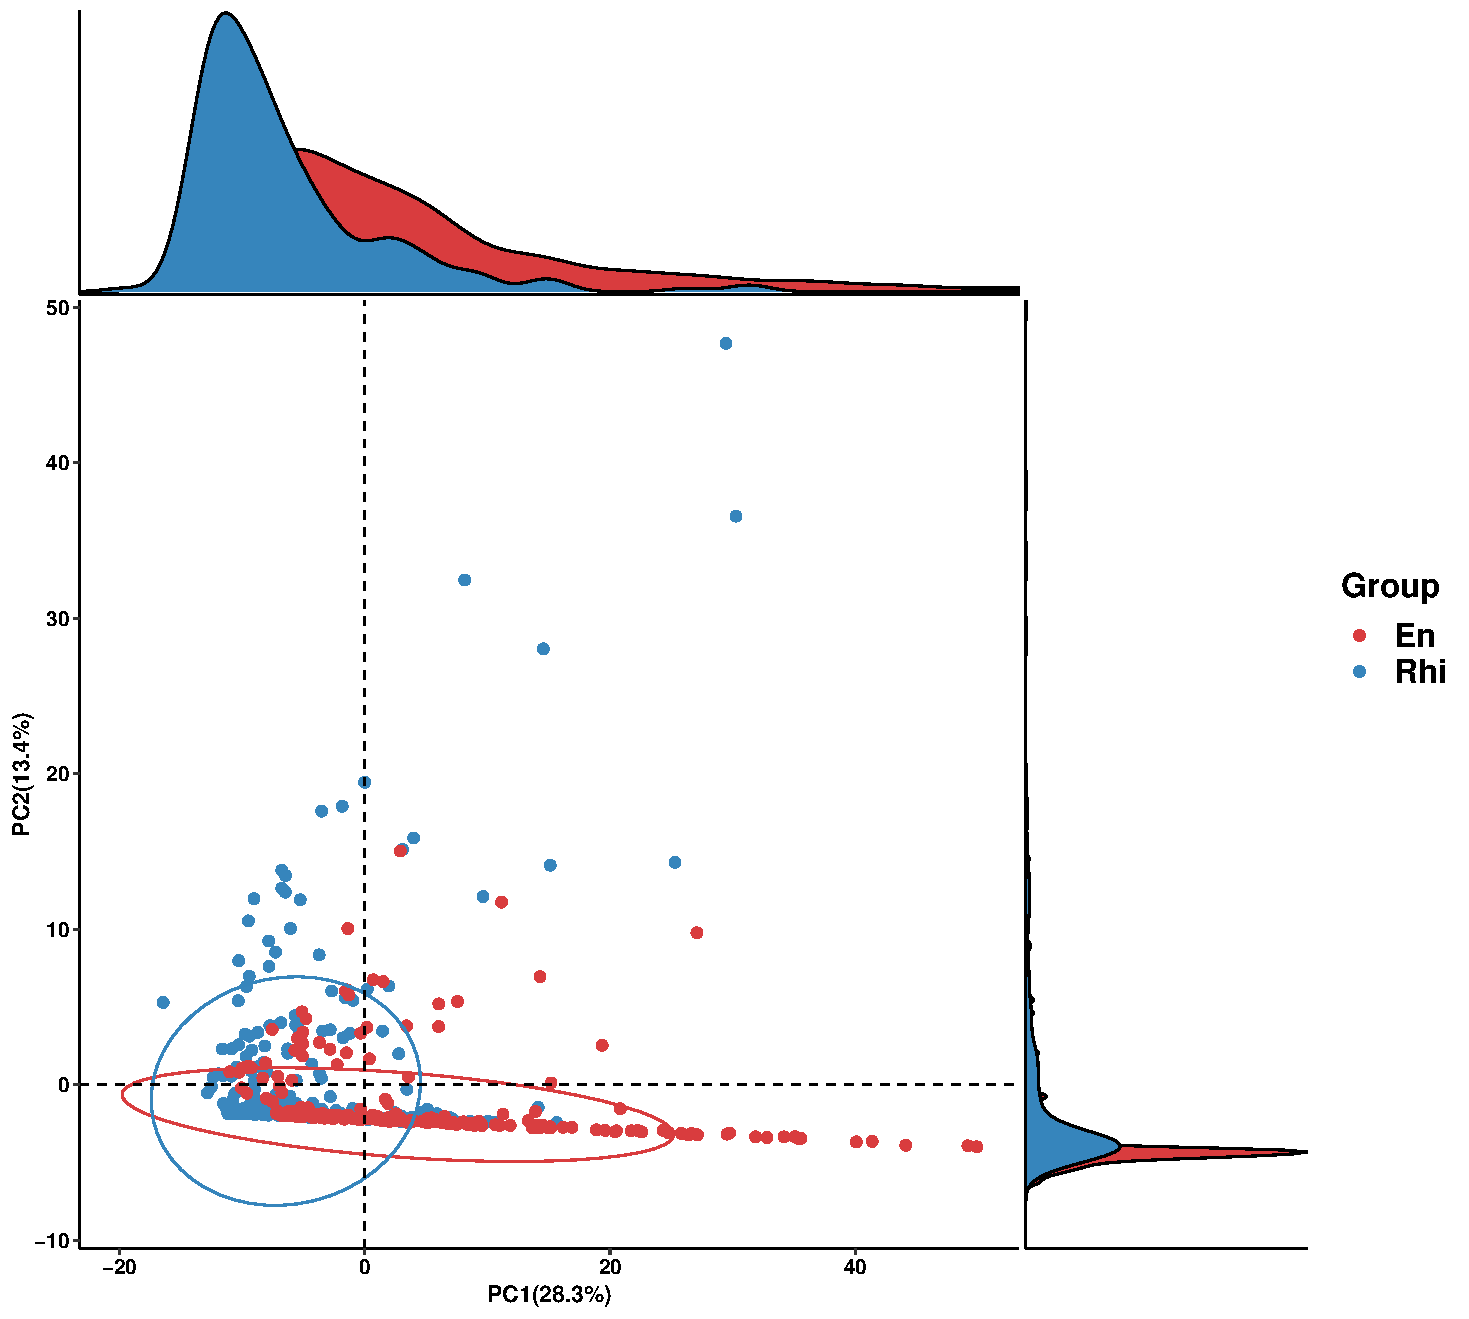
\includegraphics[width=0.5\textwidth]{img/PCA_KO.pdf}
		\caption{根内、根际微生物功能差异}
	\end{figure}

\end{frame}

	\section*{}
	\subsection*{总结}
	\begin{frame}{总结}

		\qquad 综合以上步骤,我们开发了一套在微生物层面培养、鉴定并进行功能预测的高通量方法。湿实验部分包括样本的获取、高通量培养和样本储存,干实验部分包括从二代测序下机数据到扩增子分析、物种鉴定和功能预测。
		\newline\\

		为了保证结果的可重复性,我们使用 Git 进行代码管理。
		
		代码获取:\href{https://github.com/Bluuur/BiC-Microbiome-Pipeline}{Bluuur/BiC-Microbiome-Pipeline (github.com)}
	
	\end{frame}

% ----------------- Frame -----------------

	\section*{致谢}  
	\begin{frame}
		\begin{center}
			\textcolor{darkGreen}{\huge {谢谢!\\ \quad \\ 请老师批评指正!}}
		\end{center}
	\end{frame}

\end{document}